%----------------------------------------------------------------------------------------
%	PACKAGES AND THEMES
%----------------------------------------------------------------------------------------
\documentclass[aspectratio=169,xcolor=dvipsnames]{beamer}
\usetheme{SimplePlus}

\usepackage{hyperref}
\usepackage{graphicx} % Allows including images
\usepackage{booktabs} % Allows the use of \toprule, \midrule and \bottomrule in tables
\usepackage{pdfpages}

\usepackage{lineno}
\usepackage{graphicx} 
\usepackage{subcaption}
\usepackage{amsmath}
\usepackage{booktabs}
\usepackage{float}


%----------------------------------------------------------------------------------------
%	TITLE PAGE
%----------------------------------------------------------------------------------------

\title{The Role of Media Coverage in Shaping Household Inflation Expectations: An Analysis of ECB Press Conferences and News Reporting} 

\author[authors] {Jasper Bär}

%----------------------------------------------------------------------------------------
%	PRESENTATION SLIDES
%----------------------------------------------------------------------------------------

\begin{document}

\begin{frame}[noframenumbering,plain]
    % Print the title page as the first slide
    \titlepage
\end{frame}

%------------------------------------------------
\section{First Section}
%------------------------------------------------

\begin{frame}{Main Idea}

\begin{itemize}
<<<<<<< Updated upstream
	\item How does media coverage influences inflation expectations?
	\item 
=======
\item How does media coverage influence inflation expectations?
\item Does the media inflation coverage and ECB reporting differ?
\item Can the difference between media and ECB reports explain the inflation expectation gap of the households?
>>>>>>> Stashed changes
\end{itemize}

\end{frame}

%------------------------------------------------

\begin{frame}{Model}

\begin{itemize}
<<<<<<< Updated upstream
	\item I follow Lamla and Lein (2014) and use a Bayesian Learning framework for forming my hypothesis.
	\item The central bank sends a normally distributed signal $c_t$ about the central bank inflation forecast to the media.
	\item Without the central bank the media would send a normally distributed "baseline" signal about the future inflation $s_{\nu,t}^b$ for a number of media report $V$. 
	\item The media sends a signal $s_{\nu,t}$ about the future inflation which is the weighted average of the central banks signal and the "baseline" signal. 
	\begin{align*}
s_{\nu,t} = (1-\lambda_{\nu,t}) s^b_{\nu,t} + \lambda_{\nu,t} c_t \quad 0\leq \lambda_{\nu,t} \leq 1 \\
=======
\item I follow Lamla and Lein (2014) and use a Bayesian Learning framework for forming my hypothesis.
\item The central bank sends a normally distributed signal $c_t$ about the central bank inflation forecast to the media.
\item Without the central bank, the media would send a normally distributed "baseline" signal about the future inflation $s_{\nu,t}^b$ for a number of media reports $V$.
\item The media sends a signal $s_{\nu,t}$ about the future inflation which is the weighted average of the central bank's signal and the "baseline" signal.
\begin{align*}
s_{\nu,t} = (1-\lambda_{\nu,t}) s^b_{\nu,t} + \lambda_{\nu,t} c_t \quad 0\leq \lambda_{\nu,t} \leq 1 \
>>>>>>> Stashed changes
\end{align*}
\end{itemize}

\end{frame}

%------------------------------------------------

\begin{frame}{Model}

\begin{itemize}
<<<<<<< Updated upstream
	\item Given that $s_{\nu,t}$ is a linear combination of normal random variables and assuming that $\sigma^c_t$ and $\sigma^{sb}{\nu,t}$ are independent, the media sends a normally distributed signal about $\pi{t+1}$ with $s_{\nu,t} \sim N(\mu^s_{\nu,t}, \sigma^s_{\nu,t})$, where:
\begin{equation} 
\mu_{\nu,t}^s = (1-\lambda_{\nu,t}) (\alpha_t + \Psi_t) + \lambda_{\nu,t} \Theta_t 
\end{equation}
	\item The households hold a prior belief $\gamma_t \sim N(\pi_t, \sigma^h_t)$ about the future inflation.
	\begin{align*}
s_{\nu,t} = (1-\lambda_{\nu,t}) s^b_{\nu,t} + \lambda_{\nu,t} c_t \quad 0\leq \lambda_{\nu,t} \leq 1 \\
=======
\item Given that $s_{\nu,t}$ is a linear combination of normal random variables and assuming that $\sigma^c_t$ and $\sigma^{sb}{\nu,t}$ are independent, the media sends a normally distributed signal about $\pi{t+1}$ with $s_{\nu,t} \sim N(\mu^s_{\nu,t}, \sigma^s_{\nu,t})$, where:
\begin{equation}
\mu_{\nu,t}^s = (1-\lambda_{\nu,t}) (\alpha_t + \Psi_t) + \lambda_{\nu,t} \Theta_t
\end{equation}
\item The households hold a prior belief $\gamma_t \sim N(\pi_t, \sigma^h_t)$ about the future inflation.
\item Following the Bayesian updating rule, the households' updated mean is
\begin{align*}
\mu_t = \rho_t \pi_t + (1-\rho_t)(\alpha_t(1- \bar{\lambda_t}) + \Psi_t)
>>>>>>> Stashed changes
\end{align*}
\end{itemize}

\end{frame}
<<<<<<< Updated upstream
=======
%------------------------------------------------

\begin{frame}{Model}

\begin{itemize}
	\item $B_t$ is the difference between the professional inflation forecast and the household inflation expectations. I assume that the rational inflation forecasts of the central bank and of the media are similar, i.e, $\Theta_t \approx \Psi_t$.
\begin{equation}
B_t = |\mu_t - \Psi_t| = |\rho_t \pi_t + (1-\rho_t)(\alpha_t(1- \bar{\lambda_t}) + \Psi_t) - \Psi_t|
\end{equation}
\begin{equation}
= |(1-\rho_t)(1-\bar{\lambda}_t)\alpha_t + \rho(\pi_t - \Psi_t)|
\end{equation}
	\item \textbf{Hypothesis 1:} \textit{If the media's signal is affected by a media bias, an increase in the weight given to the central bank communication by the media has an ambiguous effect on the household inflation forecasting accuracy, depending on the size of the difference between the current inflation and the rational inflation forecast.}
	\item \textbf{Hypothesis 2:} \textit{An increase of the media bias by the media has an ambiguous effect on the household inflation forecasting accuracy depending on the size of the difference between the current inflation and the rational inflation forecast.}

\end{itemize}

\end{frame}
>>>>>>> Stashed changes

%------------------------------------------------

\begin{frame}{Data}

\begin{itemize}
<<<<<<< Updated upstream
	\item Newspaper Dataset from Dpa. I could also add "Die Welt" once the datset is ready.
=======
	\item Newspaper Dataset from Dpa. I could also add "Die Welt" once the dataset is ready.
>>>>>>> Stashed changes
	\item All sentences which contain the word "Inflation" or its synonyms like "Preissteigerung" (price increase) are identified as inflation related.
	\item ECB press conferences are downloaded from the official ECB website and cleaned.
\end{itemize}

\end{frame}

%------------------------------------------------

\begin{frame}{Measuring Media Bias}

\begin{itemize}
	\item I annotated 3000 sentences from the Newspaper articles and the ECB press conferences.
	\item I used a method from Shapiro et al. (2022) based on PMI to create lexicons for the two datasets.
	\item Newspaper articles sentences are classified into "Inflation Direction" and "Inflation Sentiment".
	\item ECB press conferences are classified into "Inflation Direction".
	\item Dependency parsing is used to identify all sentences in which the ECB is directly or indirectly cited.
\end{itemize}

\end{frame}

%------------------------------------------------

\begin{frame}{Measuring Media Bias}

 \begin{figure}[!ht]
    \centering
    \setkeys{Gin}{width=\linewidth,height=6cm} %set image parameters
    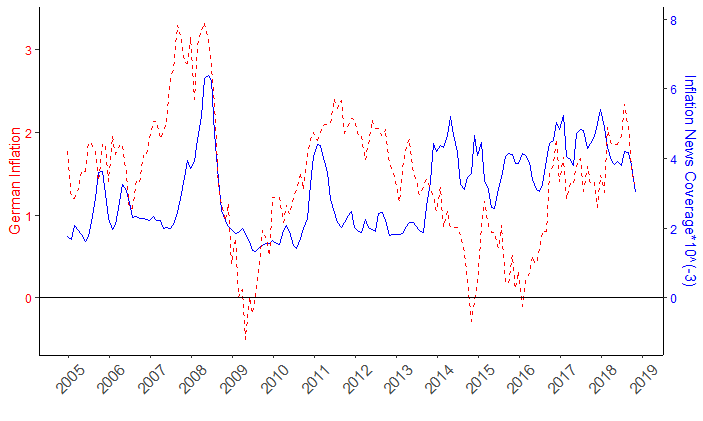
\includegraphics{Inflation_Count.png}
    \end{figure}

\end{frame}

%------------------------------------------------

\begin{frame}{Measuring Media Bias}

 \begin{figure}[!ht]
    \centering
    \setkeys{Gin}{width=\linewidth,height=6cm} %set image parameters
    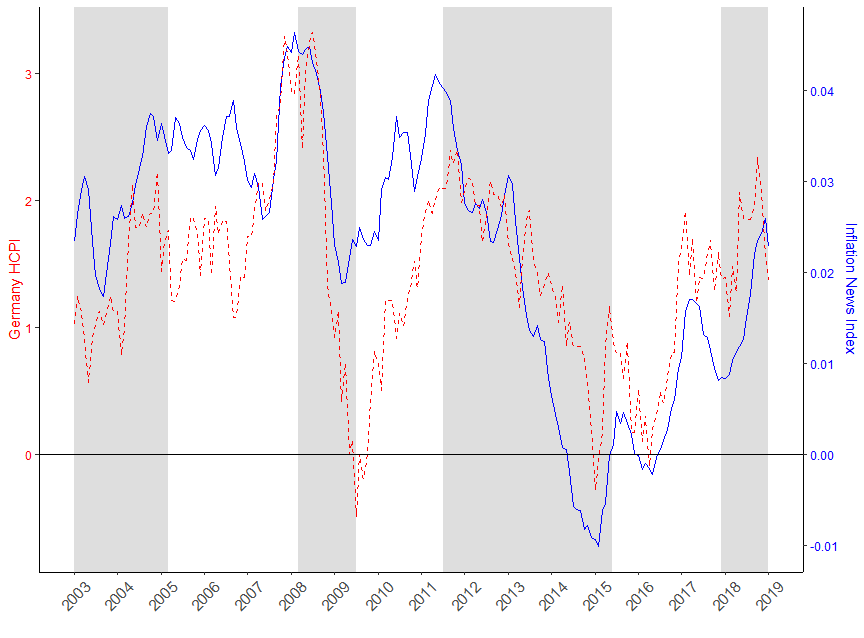
\includegraphics{Inflation_Sentiment_Direction.png}
    \label{Inflation_Sentiment_Direction}
    \end{figure}

\end{frame}

%------------------------------------------------


\begin{frame}{Measuring Media Bias}

<<<<<<< Updated upstream
Plots
=======
   \begin{figure}[!ht]
    \centering
    \setkeys{Gin}{width=\linewidth,height=6cm} %set image parameters
    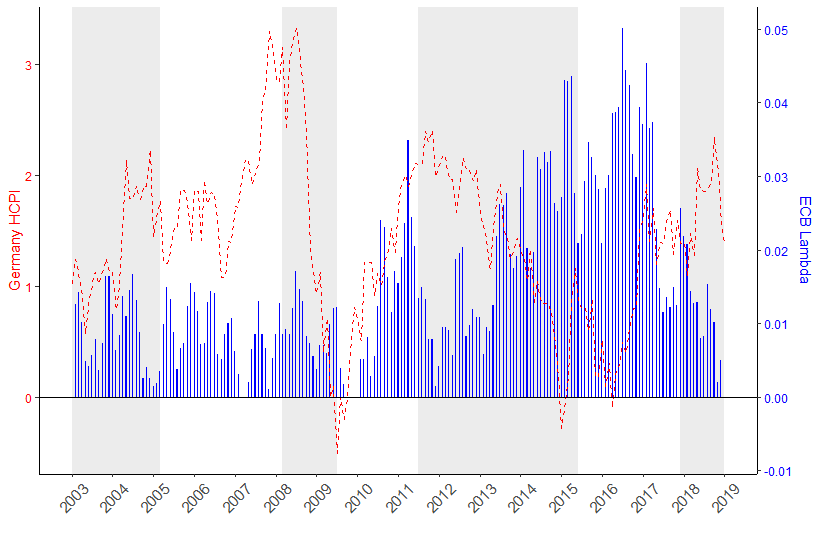
\includegraphics{ECB Lambda.png}
    \end{figure}
>>>>>>> Stashed changes

\end{frame}

%------------------------------------------------

<<<<<<< Updated upstream
=======
\begin{frame}{Measuring Media Bias}

   \begin{figure}[!ht]
    \centering
    \setkeys{Gin}{width=\linewidth,height=6cm} %set image parameters
    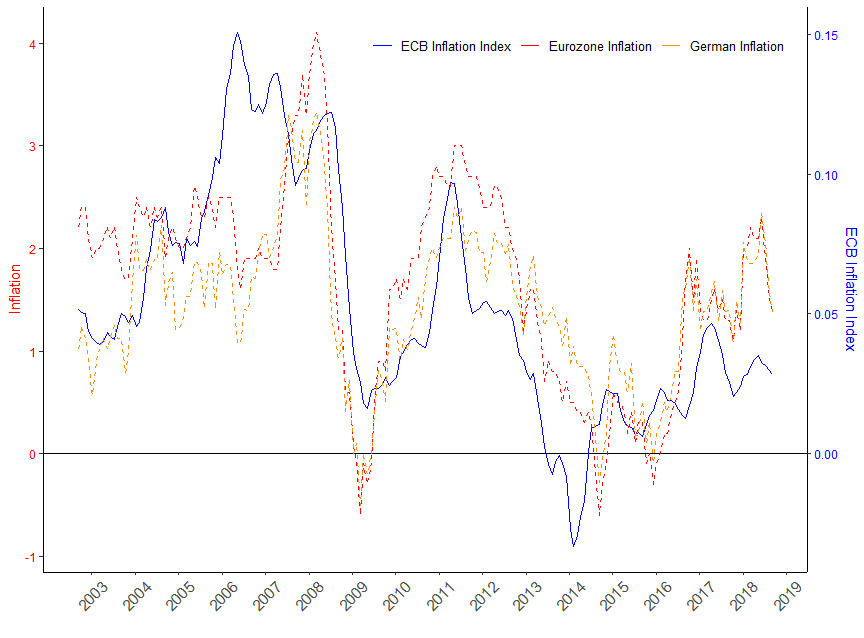
\includegraphics{ECB_inf_inf.png}
    \end{figure}

\end{frame}

%------------------------------------------------


>>>>>>> Stashed changes
\begin{frame}{Inflation Expectations Gap}

\begin{itemize}
\item I follow Lamla and Lein (2014) and measure the inflation expectations gap as the quantified inflation forecast and the professional one-year-ahead forecasts.
\item Several quantification methods exist. 
<<<<<<< Updated upstream
\item Quantification methods are barely mentioned after 2014. Why?
=======
\item Quantification methods are barely mentioned in the literature after 2014. Why?
>>>>>>> Stashed changes
\end{itemize}

\end{frame}

%------------------------------------------------

\begin{frame}{Inflation Expectations Gap}

<<<<<<< Updated upstream
Plot
=======
  \begin{figure}[!ht]
    \centering
    \setkeys{Gin}{width=\linewidth,height=6cm} %set image parameters
    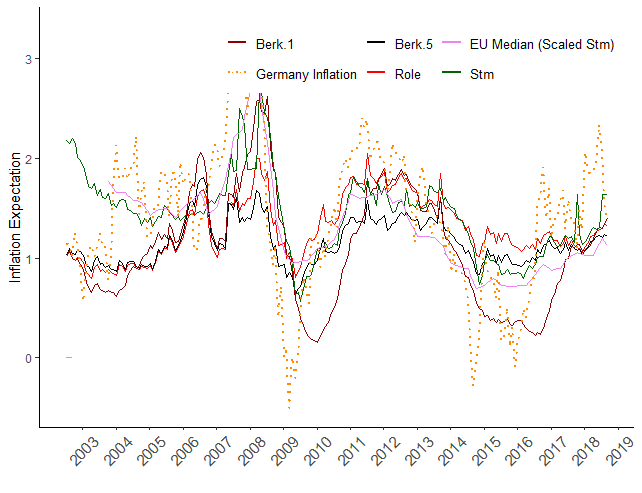
\includegraphics{Household_Inf_Exp.png}
    \end{figure}

\end{frame}

%------------------------------------------------

\begin{frame}{Inflation Expectations Gap}

 \begin{itemize}
 \item I base the professional inflation forecast on Reuters Poll data
 \item To get the one-year-ahead forecast I follow Dovern et al. 2012 and transform the forecast as follows: for month m of a given year $t$, the expectation of inflation is defined as (13-$m$)/12 times the forecast for year $t$ plus (m-1)/12 times the forecast for year $t$ + 1.
 \end{itemize}
>>>>>>> Stashed changes

\end{frame}

%------------------------------------------------

<<<<<<< Updated upstream
=======
\begin{frame}{Preliminary Results}

 \begin{itemize}
 \item To get the media bias, I regress the ECB inflation index on the inflation news index.
 \item I directly use the occurrence of ECB related inflation as a measure for $\lambda_t$.
 \end{itemize}

\end{frame}

%------------------------------------------------

\begin{frame}{Inflation Expectations Gap}

  \begin{figure}[!ht]
    \centering
    \setkeys{Gin}{width=\linewidth,height=6cm} %set image parameters
    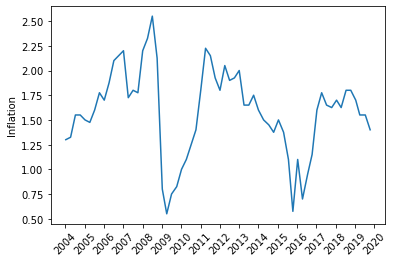
\includegraphics{Reuter_Poll.png}
    \end{figure}

\end{frame}

%------------------------------------------------

\begin{frame}{Inflation Expectations Gap}

  \begin{table}[!ht]
  \small
\centering 
  \caption{Inflation Expectation Gap Stm-Reuter} 
  \label{tab:Inflation Expectation Gap Stm-Reuter}
\begin{tabular}{l*{6}{c}}   
\toprule
                    & (1) & (2) & (3) & (4) & (5) \\
\midrule
$B_{t-1}$           &     & -0.134 & -0.123 & -0.175 & -0.134 \\
                    &     & (0.101) & (0.101) & (0.108) & (0.101) \\
$\pi_{t-1}$         &     & 0.029 & 0.038 & 0.036 & 0.029 \\
                    &     & (0.054) & (0.048) & (0.048) & (0.054) \\
$\tilde{V_t}$       & 8.542 & 16.346 & 10.648 & 24.031 & 21.087 \\
                    & (18.605) & (17.296) & (17.226) & (16.387) & (16.438) \\
$\tilde{\alpha_t}$  &     &     & 1.227 &     & 1.218 \\
                    &     &     & (1.118) &     & (1.074) \\
$\tilde{\lambda_t}$ &     &     &     & -2.369 & -2.340 \\
                    &     &     &     & (1.560) & (1.453) \\
$Constant$          & 0.299*** & 0.230*** & 0.273*** & 0.334*** & 0.328*** \\
                    & (0.041) & (0.075) & (0.079) & (0.083) & (0.081) \\
\midrule
$R^2$               & 0.003 & 0.030 & 0.090 & 0.076 & 0.110 \\
\bottomrule
\end{tabular} 
\parbox{0.8\textwidth}{\centering \small *** p $<$ 0.01, ** p $<$ 0.05, * p $<$ 0.1.}
\end{table}

\end{frame}

%------------------------------------------------

\begin{frame}{Inflation Expectations Gap}

\begin{table}[!ht]
\small
\centering 
  \caption{Inflation Expectation Gap Berk 5-Reuter} 
  \label{tab:Inflation Expectation Gap Berk 5-Reuter}
\begin{tabular}{l*{6}{c}}   
\toprule
                    & (1) & (2) & (3) & (4) & (5) \\
\midrule
$B_{t-1}$           &     & -0.239 & -0.214 & -0.269 & -0.239 \\
                    &     & (0.163) & (0.171) & (0.189) & (0.163) \\
$\pi_{t-1}$         &     & 0.117*** & 0.131*** & 0.140*** & 0.117*** \\
                    &     & (0.030) & (0.035) & (0.045) & (0.030) \\
$\tilde{V_t}$       & 11.181 & 30.037 & 19.441 & 46.170** & 38.676** \\
                    & (30.345) & (22.872) & (18.464) & (19.710) & (16.863) \\
$\tilde{\alpha_t}$  &     &     & 2.723*** &     & 2.725*** \\
                    &     &     & (0.695) &     & (0.627) \\
$\tilde{\lambda_t}$ &     &     &     & -4.304*** & -4.313*** \\
                    &     &     &     & (1.604) & (1.431) \\
$Constant$          & 0.447*** & 0.281*** & 0.342*** & 0.432*** & 0.442*** \\
                    & (0.057) & (0.097) & (0.094) & (0.114) & (0.086) \\
\midrule
$R^2$               & 0.004 & 0.124 & 0.300 & 0.217 & 0.351 \\
\bottomrule
\end{tabular} 
\parbox{0.8\textwidth}{\centering \small *** p $<$ 0.01, ** p $<$ 0.05, * p $<$ 0.1.}
\end{table}

\end{frame}

%------------------------------------------------

\begin{frame}{Inflation Expectations Gap}

\begin{table}[!ht]
\small
\centering 
  \caption{Inflation Expectation Gap Role-Reuter} 
  \label{tab:Inflation Expectation Gap Role-Reuter}
\begin{tabular}{l*{6}{c}}   
\toprule
                    & (1) & (2) & (3) & (4) & (5) \\
\midrule
$B_{t-1}$           &     & 0.283*** & 0.342*** & 0.336*** & 0.283*** \\
                    &     & (0.094) & (0.097) & (0.122) & (0.094) \\
$\pi_{t-1}$         &     & 0.013 & 0.024 & 0.031 & 0.013 \\
                    &     & (0.031) & (0.033) & (0.036) & (0.031) \\
$\tilde{V_t}$       & 4.896 & 16.201 & 9.442 & 33.589* & 25.693 \\
                    & (27.311) & (24.768) & (17.531) & (19.324) & (16.457) \\
$\tilde{\alpha_t}$  &     &     & 3.079*** &     & 3.136*** \\
                    &     &     & (0.671) &     & (0.635) \\
$\tilde{\lambda_t}$ &     &     &     & -3.363** & -3.702*** \\
                    &     &     &     & (1.646) & (1.406) \\
$Constant$          & 0.351*** & 0.251*** & 0.183*** & 0.240*** & 0.279*** \\
                    & (0.055) & (0.064) & (0.058) & (0.078) & (0.066) \\
\midrule
$R^2$               & 0.001 & 0.046 & 0.368 & 0.221 & 0.403 \\
\bottomrule
\end{tabular} 
\parbox{0.8\textwidth}{\centering \small *** p $<$ 0.01, ** p $<$ 0.05, * p $<$ 0.1.}
\end{table}

\end{frame}

%------------------------------------------------


>>>>>>> Stashed changes
\end{document}